\documentclass[1p]{elsarticle_modified}
%\bibliographystyle{elsarticle-num}

%\usepackage[colorlinks]{hyperref}
%\usepackage{abbrmath_seonhwa} %\Abb, \Ascr, \Acal ,\Abf, \Afrak
\usepackage{amsfonts}
\usepackage{amssymb}
\usepackage{amsmath}
\usepackage{amsthm}
\usepackage{scalefnt}
\usepackage{amsbsy}
\usepackage{kotex}
\usepackage{caption}
\usepackage{subfig}
\usepackage{color}
\usepackage{graphicx}
\usepackage{xcolor} %% white, black, red, green, blue, cyan, magenta, yellow
\usepackage{float}
\usepackage{setspace}
\usepackage{hyperref}

\usepackage{tikz}
\usetikzlibrary{arrows}

\usepackage{multirow}
\usepackage{array} % fixed length table
\usepackage{hhline}

%%%%%%%%%%%%%%%%%%%%%
\makeatletter
\renewcommand*\env@matrix[1][\arraystretch]{%
	\edef\arraystretch{#1}%
	\hskip -\arraycolsep
	\let\@ifnextchar\new@ifnextchar
	\array{*\c@MaxMatrixCols c}}
\makeatother %https://tex.stackexchange.com/questions/14071/how-can-i-increase-the-line-spacing-in-a-matrix
%%%%%%%%%%%%%%%

\usepackage[normalem]{ulem}

\newcommand{\msout}[1]{\ifmmode\text{\sout{\ensuremath{#1}}}\else\sout{#1}\fi}
%SOURCE: \msout is \stkout macro in https://tex.stackexchange.com/questions/20609/strikeout-in-math-mode

\newcommand{\cancel}[1]{
	\ifmmode
	{\color{red}\msout{#1}}
	\else
	{\color{red}\sout{#1}}
	\fi
}

\newcommand{\add}[1]{
	{\color{blue}\uwave{#1}}
}

\newcommand{\replace}[2]{
	\ifmmode
	{\color{red}\msout{#1}}{\color{blue}\uwave{#2}}
	\else
	{\color{red}\sout{#1}}{\color{blue}\uwave{#2}}
	\fi
}

\newcommand{\Sol}{\mathcal{S}} %segment
\newcommand{\D}{D} %diagram
\newcommand{\A}{\mathcal{A}} %arc


%%%%%%%%%%%%%%%%%%%%%%%%%%%%%5 test

\def\sl{\operatorname{\textup{SL}}(2,\Cbb)}
\def\psl{\operatorname{\textup{PSL}}(2,\Cbb)}
\def\quan{\mkern 1mu \triangleright \mkern 1mu}

\theoremstyle{definition}
\newtheorem{thm}{Theorem}[section]
\newtheorem{prop}[thm]{Proposition}
\newtheorem{lem}[thm]{Lemma}
\newtheorem{ques}[thm]{Question}
\newtheorem{cor}[thm]{Corollary}
\newtheorem{defn}[thm]{Definition}
\newtheorem{exam}[thm]{Example}
\newtheorem{rmk}[thm]{Remark}
\newtheorem{alg}[thm]{Algorithm}

\newcommand{\I}{\sqrt{-1}}
\begin{document}

%\begin{frontmatter}
%
%\title{Boundary parabolic representations of knots up to 8 crossings}
%
%%% Group authors per affiliation:
%\author{Yunhi Cho} 
%\address{Department of Mathematics, University of Seoul, Seoul, Korea}
%\ead{yhcho@uos.ac.kr}
%
%
%\author{Seonhwa Kim} %\fnref{s_kim}}
%\address{Center for Geometry and Physics, Institute for Basic Science, Pohang, 37673, Korea}
%\ead{ryeona17@ibs.re.kr}
%
%\author{Hyuk Kim}
%\address{Department of Mathematical Sciences, Seoul National University, Seoul 08826, Korea}
%\ead{hyukkim@snu.ac.kr}
%
%\author{Seokbeom Yoon}
%\address{Department of Mathematical Sciences, Seoul National University, Seoul, 08826,  Korea}
%\ead{sbyoon15@snu.ac.kr}
%
%\begin{abstract}
%We find all boundary parabolic representation of knots up to 8 crossings.
%
%\end{abstract}
%\begin{keyword}
%    \MSC[2010] 57M25 
%\end{keyword}
%
%\end{frontmatter}

%\linenumbers
%\tableofcontents
%
\newcommand\colored[1]{\textcolor{white}{\rule[-0.35ex]{0.8em}{1.4ex}}\kern-0.8em\color{red} #1}%
%\newcommand\colored[1]{\textcolor{white}{ #1}\kern-2.17ex	\textcolor{white}{ #1}\kern-1.81ex	\textcolor{white}{ #1}\kern-2.15ex\color{red}#1	}

{\Large $\underline{12a_{1063}~(K12a_{1063})}$}

\setlength{\tabcolsep}{10pt}
\renewcommand{\arraystretch}{1.6}
\vspace{1cm}\begin{tabular}{m{100pt}>{\centering\arraybackslash}m{274pt}}
\multirow{5}{120pt}{
	\centering
	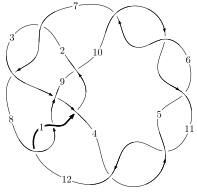
\includegraphics[width=112pt]{../../../GIT/diagram.site/Diagrams/png/1864_12a_1063.png}\\
\ \ \ A knot diagram\footnotemark}&
\allowdisplaybreaks
\textbf{Linearized knot diagam} \\
\cline{2-2}
 &
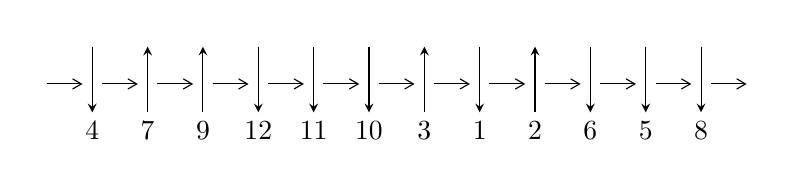
\begin{tikzpicture}[x=20pt, y=17pt]
	% nodes
	\node (C0) at (0, 0) {};
	\node (C1) at (1, 0) {};
	\node (C1U) at (1, +1) {};
	\node (C1D) at (1, -1) {4};

	\node (C2) at (2, 0) {};
	\node (C2U) at (2, +1) {};
	\node (C2D) at (2, -1) {7};

	\node (C3) at (3, 0) {};
	\node (C3U) at (3, +1) {};
	\node (C3D) at (3, -1) {9};

	\node (C4) at (4, 0) {};
	\node (C4U) at (4, +1) {};
	\node (C4D) at (4, -1) {12};

	\node (C5) at (5, 0) {};
	\node (C5U) at (5, +1) {};
	\node (C5D) at (5, -1) {11};

	\node (C6) at (6, 0) {};
	\node (C6U) at (6, +1) {};
	\node (C6D) at (6, -1) {10};

	\node (C7) at (7, 0) {};
	\node (C7U) at (7, +1) {};
	\node (C7D) at (7, -1) {3};

	\node (C8) at (8, 0) {};
	\node (C8U) at (8, +1) {};
	\node (C8D) at (8, -1) {1};

	\node (C9) at (9, 0) {};
	\node (C9U) at (9, +1) {};
	\node (C9D) at (9, -1) {2};

	\node (C10) at (10, 0) {};
	\node (C10U) at (10, +1) {};
	\node (C10D) at (10, -1) {6};

	\node (C11) at (11, 0) {};
	\node (C11U) at (11, +1) {};
	\node (C11D) at (11, -1) {5};

	\node (C12) at (12, 0) {};
	\node (C12U) at (12, +1) {};
	\node (C12D) at (12, -1) {8};
	\node (C13) at (13, 0) {};

	% arrows
	\draw[->,>={angle 60}]
	(C0) edge (C1) (C1) edge (C2) (C2) edge (C3) (C3) edge (C4) (C4) edge (C5) (C5) edge (C6) (C6) edge (C7) (C7) edge (C8) (C8) edge (C9) (C9) edge (C10) (C10) edge (C11) (C11) edge (C12) (C12) edge (C13) ;	\draw[->,>=stealth]
	(C1U) edge (C1D) (C2D) edge (C2U) (C3D) edge (C3U) (C4U) edge (C4D) (C5U) edge (C5D) (C6U) edge (C6D) (C7D) edge (C7U) (C8U) edge (C8D) (C9D) edge (C9U) (C10U) edge (C10D) (C11U) edge (C11D) (C12U) edge (C12D) ;
	\end{tikzpicture} \\
\hhline{~~} \\& 
\textbf{Solving Sequence} \\ \cline{2-2} 
 &
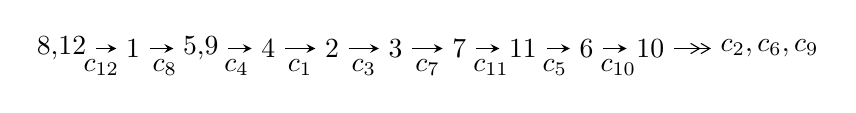
\begin{tikzpicture}[x=23pt, y=7pt]
	% node
	\node (A0) at (-1/8, 0) {8,12};
	\node (A1) at (1, 0) {1};
	\node (A2) at (33/16, 0) {5,9};
	\node (A3) at (25/8, 0) {4};
	\node (A4) at (33/8, 0) {2};
	\node (A5) at (41/8, 0) {3};
	\node (A6) at (49/8, 0) {7};
	\node (A7) at (57/8, 0) {11};
	\node (A8) at (65/8, 0) {6};
	\node (A9) at (73/8, 0) {10};
	\node (C1) at (1/2, -1) {$c_{12}$};
	\node (C2) at (3/2, -1) {$c_{8}$};
	\node (C3) at (21/8, -1) {$c_{4}$};
	\node (C4) at (29/8, -1) {$c_{1}$};
	\node (C5) at (37/8, -1) {$c_{3}$};
	\node (C6) at (45/8, -1) {$c_{7}$};
	\node (C7) at (53/8, -1) {$c_{11}$};
	\node (C8) at (61/8, -1) {$c_{5}$};
	\node (C9) at (69/8, -1) {$c_{10}$};
	\node (A10) at (11, 0) {$c_{2},c_{6},c_{9}$};

	% edge
	\draw[->,>=stealth]	
	(A0) edge (A1) (A1) edge (A2) (A2) edge (A3) (A3) edge (A4) (A4) edge (A5) (A5) edge (A6) (A6) edge (A7) (A7) edge (A8) (A8) edge (A9) ;
	\draw[->>,>={angle 60}]	
	(A9) edge (A10);
\end{tikzpicture} \\ 

\end{tabular} \\

\footnotetext{
The image of knot diagram is generated by the software ``\textbf{Draw programme}" developed by Andrew Bartholomew(\url{http://www.layer8.co.uk/maths/draw/index.htm\#Running-draw}), where we modified some parts for our purpose(\url{https://github.com/CATsTAILs/LinksPainter}).
}\phantom \\ \newline 
\centering \textbf{Ideals for irreducible components\footnotemark of $X_{\text{par}}$} 
 
\begin{align*}
I^u_{1}&=\langle 
6.41268\times10^{106} u^{66}+5.37842\times10^{106} u^{65}+\cdots+7.96827\times10^{105} b+2.18486\times10^{108},\\
\phantom{I^u_{1}}&\phantom{= \langle  }-5.09982\times10^{109} u^{66}-3.33786\times10^{109} u^{65}+\cdots+1.77932\times10^{109} a-1.54505\times10^{111},\\
\phantom{I^u_{1}}&\phantom{= \langle  }u^{67}-18 u^{65}+\cdots+34 u-29\rangle \\
I^u_{2}&=\langle 
- u^{11}-2 u^{10}+3 u^9+8 u^8-7 u^7-21 u^6+7 u^5+27 u^4-4 u^3-20 u^2+b+u+5,\\
\phantom{I^u_{2}}&\phantom{= \langle  }-2 u^{12}+10 u^{10}+2 u^9-32 u^8-4 u^7+58 u^6+6 u^5-66 u^4-2 u^3+41 u^2+a-12,\\
\phantom{I^u_{2}}&\phantom{= \langle  }u^{13}+u^{12}-4 u^{11}-5 u^{10}+11 u^9+13 u^8-16 u^7-19 u^6+14 u^5+15 u^4-6 u^3-6 u^2+u+1\rangle \\
\\
\end{align*}
\raggedright * 2 irreducible components of $\dim_{\mathbb{C}}=0$, with total 80 representations.\\
\footnotetext{All coefficients of polynomials are rational numbers. But the coefficients are sometimes approximated in decimal forms when there is not enough margin.}
\newpage
\renewcommand{\arraystretch}{1}
\centering \section*{I. $I^u_{1}= \langle 6.41\times10^{106} u^{66}+5.38\times10^{106} u^{65}+\cdots+7.97\times10^{105} b+2.18\times10^{108},\;-5.10\times10^{109} u^{66}-3.34\times10^{109} u^{65}+\cdots+1.78\times10^{109} a-1.55\times10^{111},\;u^{67}-18 u^{65}+\cdots+34 u-29 \rangle$}
\flushleft \textbf{(i) Arc colorings}\\
\begin{tabular}{m{7pt} m{180pt} m{7pt} m{180pt} }
\flushright $a_{8}=$&$\begin{pmatrix}0\\u\end{pmatrix}$ \\
\flushright $a_{12}=$&$\begin{pmatrix}1\\0\end{pmatrix}$ \\
\flushright $a_{1}=$&$\begin{pmatrix}1\\u^2\end{pmatrix}$ \\
\flushright $a_{5}=$&$\begin{pmatrix}2.86617 u^{66}+1.87592 u^{65}+\cdots+26.5482 u+86.8341\\-8.04777 u^{66}-6.74979 u^{65}+\cdots+1.01965 u-274.195\end{pmatrix}$ \\
\flushright $a_{9}=$&$\begin{pmatrix}- u\\- u^3+u\end{pmatrix}$ \\
\flushright $a_{4}=$&$\begin{pmatrix}-5.18160 u^{66}-4.87387 u^{65}+\cdots+27.5678 u-187.361\\-8.04777 u^{66}-6.74979 u^{65}+\cdots+1.01965 u-274.195\end{pmatrix}$ \\
\flushright $a_{2}=$&$\begin{pmatrix}-0.569565 u^{66}+0.302604 u^{65}+\cdots-60.1340 u+38.1233\\-5.45740 u^{66}-5.15294 u^{65}+\cdots+17.0431 u-197.550\end{pmatrix}$ \\
\flushright $a_{3}=$&$\begin{pmatrix}1.53537 u^{66}+0.976716 u^{65}+\cdots+16.9891 u+52.7642\\-10.1163 u^{66}-8.67159 u^{65}+\cdots+7.47077 u-344.653\end{pmatrix}$ \\
\flushright $a_{7}=$&$\begin{pmatrix}1.29876 u^{66}+0.433635 u^{65}+\cdots+24.4829 u+22.4634\\-6.76250 u^{66}-5.55933 u^{65}+\cdots-10.3127 u-235.152\end{pmatrix}$ \\
\flushright $a_{11}=$&$\begin{pmatrix}-8.09315 u^{66}-7.31257 u^{65}+\cdots+4.35672 u-276.655\\-1.69292 u^{66}-1.39081 u^{65}+\cdots-4.92421 u-54.8481\end{pmatrix}$ \\
\flushright $a_{6}=$&$\begin{pmatrix}4.79638 u^{66}+3.91190 u^{65}+\cdots+9.42862 u+183.767\\9.31661 u^{66}+7.79591 u^{65}+\cdots+0.327753 u+313.089\end{pmatrix}$ \\
\flushright $a_{10}=$&$\begin{pmatrix}3.20540 u^{66}+2.54543 u^{65}+\cdots-1.99013 u+114.771\\3.37305 u^{66}+3.10208 u^{65}+\cdots-4.99752 u+106.804\end{pmatrix}$\\&\end{tabular}
\flushleft \textbf{(ii) Obstruction class $= -1$}\\~\\
\flushleft \textbf{(iii) Cusp Shapes $= -2.24398 u^{66}-2.83903 u^{65}+\cdots+14.5192 u-13.8222$}\\~\\
\newpage\renewcommand{\arraystretch}{1}
\flushleft \textbf{(iv) u-Polynomials at the component}\newline \\
\begin{tabular}{m{50pt}|m{274pt}}
Crossings & \hspace{64pt}u-Polynomials at each crossing \\
\hline $$\begin{aligned}c_{1}\end{aligned}$$&$\begin{aligned}
&u^{67}-11 u^{66}+\cdots+187 u-13
\end{aligned}$\\
\hline $$\begin{aligned}c_{2},c_{7}\end{aligned}$$&$\begin{aligned}
&u^{67}-28 u^{65}+\cdots-926 u-317
\end{aligned}$\\
\hline $$\begin{aligned}c_{3}\end{aligned}$$&$\begin{aligned}
&u^{67}- u^{66}+\cdots-5 u-1
\end{aligned}$\\
\hline $$\begin{aligned}c_{4},c_{5},c_{6}\\c_{10},c_{11}\end{aligned}$$&$\begin{aligned}
&u^{67}+u^{66}+\cdots+15 u-1
\end{aligned}$\\
\hline $$\begin{aligned}c_{8},c_{12}\end{aligned}$$&$\begin{aligned}
&u^{67}-18 u^{65}+\cdots+34 u-29
\end{aligned}$\\
\hline $$\begin{aligned}c_{9}\end{aligned}$$&$\begin{aligned}
&u^{67}+3 u^{66}+\cdots+82237 u+97193
\end{aligned}$\\
\hline
\end{tabular}\\~\\
\newpage\renewcommand{\arraystretch}{1}
\flushleft \textbf{(v) Riley Polynomials at the component}\newline \\
\begin{tabular}{m{50pt}|m{274pt}}
Crossings & \hspace{64pt}Riley Polynomials at each crossing \\
\hline $$\begin{aligned}c_{1}\end{aligned}$$&$\begin{aligned}
&y^{67}+5 y^{66}+\cdots-3199 y-169
\end{aligned}$\\
\hline $$\begin{aligned}c_{2},c_{7}\end{aligned}$$&$\begin{aligned}
&y^{67}-56 y^{66}+\cdots+1949858 y-100489
\end{aligned}$\\
\hline $$\begin{aligned}c_{3}\end{aligned}$$&$\begin{aligned}
&y^{67}+5 y^{66}+\cdots+13 y-1
\end{aligned}$\\
\hline $$\begin{aligned}c_{4},c_{5},c_{6}\\c_{10},c_{11}\end{aligned}$$&$\begin{aligned}
&y^{67}+93 y^{66}+\cdots+75 y-1
\end{aligned}$\\
\hline $$\begin{aligned}c_{8},c_{12}\end{aligned}$$&$\begin{aligned}
&y^{67}-36 y^{66}+\cdots+4694 y-841
\end{aligned}$\\
\hline $$\begin{aligned}c_{9}\end{aligned}$$&$\begin{aligned}
&y^{67}-31 y^{66}+\cdots+176544321833 y-9446479249
\end{aligned}$\\
\hline
\end{tabular}\\~\\
\newpage\flushleft \textbf{(vi) Complex Volumes and Cusp Shapes}
$$\begin{array}{c|c|c}  
\text{Solutions to }I^u_{1}& \I (\text{vol} + \sqrt{-1}CS) & \text{Cusp shape}\\
 \hline 
\begin{aligned}
u &= \phantom{-}0.911539 + 0.421875 I \\
a &= -0.068762 + 0.784351 I \\
b &= \phantom{-}0.379133 - 1.265230 I\end{aligned}
 & \phantom{-}6.39745 - 0.28170 I & \phantom{-}3.68167 + 1.63128 I \\ \hline\begin{aligned}
u &= \phantom{-}0.911539 - 0.421875 I \\
a &= -0.068762 - 0.784351 I \\
b &= \phantom{-}0.379133 + 1.265230 I\end{aligned}
 & \phantom{-}6.39745 + 0.28170 I & \phantom{-}3.68167 - 1.63128 I \\ \hline\begin{aligned}
u &= -0.957914 + 0.261576 I \\
a &= -0.867716 + 0.026848 I \\
b &= -0.344734 - 0.548883 I\end{aligned}
 & -2.09647 + 1.32539 I & -5.24417 + 2.03553 I \\ \hline\begin{aligned}
u &= -0.957914 - 0.261576 I \\
a &= -0.867716 - 0.026848 I \\
b &= -0.344734 + 0.548883 I\end{aligned}
 & -2.09647 - 1.32539 I & -5.24417 - 2.03553 I \\ \hline\begin{aligned}
u &= \phantom{-}0.941880 + 0.411762 I \\
a &= \phantom{-}2.83735 - 1.30126 I \\
b &= -0.00731 + 1.74185 I\end{aligned}
 & \phantom{-}16.3104 + 0.6556 I & \phantom{-0.000000 } 0 \\ \hline\begin{aligned}
u &= \phantom{-}0.941880 - 0.411762 I \\
a &= \phantom{-}2.83735 + 1.30126 I \\
b &= -0.00731 - 1.74185 I\end{aligned}
 & \phantom{-}16.3104 - 0.6556 I & \phantom{-0.000000 } 0 \\ \hline\begin{aligned}
u &= -0.933354 + 0.492729 I \\
a &= -1.87664 - 0.85621 I \\
b &= -0.11584 + 1.74926 I\end{aligned}
 & \phantom{-}16.8834 + 5.6261 I & \phantom{-0.000000 } 0 \\ \hline\begin{aligned}
u &= -0.933354 - 0.492729 I \\
a &= -1.87664 + 0.85621 I \\
b &= -0.11584 - 1.74926 I\end{aligned}
 & \phantom{-}16.8834 - 5.6261 I & \phantom{-0.000000 } 0 \\ \hline\begin{aligned}
u &= \phantom{-}0.044204 + 0.937111 I \\
a &= \phantom{-}0.36495 + 2.34631 I \\
b &= \phantom{-}0.01639 - 1.74788 I\end{aligned}
 & \phantom{-}14.4001 + 2.3576 I & \phantom{-}2.94594 - 2.68766 I \\ \hline\begin{aligned}
u &= \phantom{-}0.044204 - 0.937111 I \\
a &= \phantom{-}0.36495 - 2.34631 I \\
b &= \phantom{-}0.01639 + 1.74788 I\end{aligned}
 & \phantom{-}14.4001 - 2.3576 I & \phantom{-}2.94594 + 2.68766 I\\
 \hline 
 \end{array}$$\newpage$$\begin{array}{c|c|c}  
\text{Solutions to }I^u_{1}& \I (\text{vol} + \sqrt{-1}CS) & \text{Cusp shape}\\
 \hline 
\begin{aligned}
u &= \phantom{-}0.213053 + 0.888666 I \\
a &= \phantom{-}0.231539 - 0.140350 I \\
b &= -0.496535 + 0.391220 I\end{aligned}
 & \phantom{-}3.80122 + 3.48677 I & \phantom{-}1.50459 - 6.08806 I \\ \hline\begin{aligned}
u &= \phantom{-}0.213053 - 0.888666 I \\
a &= \phantom{-}0.231539 + 0.140350 I \\
b &= -0.496535 - 0.391220 I\end{aligned}
 & \phantom{-}3.80122 - 3.48677 I & \phantom{-}1.50459 + 6.08806 I \\ \hline\begin{aligned}
u &= -0.846245 + 0.321552 I \\
a &= \phantom{-}0.61208 + 2.38869 I \\
b &= \phantom{-}0.093534 - 1.199810 I\end{aligned}
 & \phantom{-}6.13436 + 3.42440 I & \phantom{-}3.18390 - 7.59222 I \\ \hline\begin{aligned}
u &= -0.846245 - 0.321552 I \\
a &= \phantom{-}0.61208 - 2.38869 I \\
b &= \phantom{-}0.093534 + 1.199810 I\end{aligned}
 & \phantom{-}6.13436 - 3.42440 I & \phantom{-}3.18390 + 7.59222 I \\ \hline\begin{aligned}
u &= -0.820163 + 0.327205 I \\
a &= \phantom{-}2.81348 + 0.85529 I \\
b &= -0.036223 - 1.035500 I\end{aligned}
 & \phantom{-}6.25055 - 0.48911 I & \phantom{-}3.45164 - 1.01139 I \\ \hline\begin{aligned}
u &= -0.820163 - 0.327205 I \\
a &= \phantom{-}2.81348 - 0.85529 I \\
b &= -0.036223 + 1.035500 I\end{aligned}
 & \phantom{-}6.25055 + 0.48911 I & \phantom{-}3.45164 + 1.01139 I \\ \hline\begin{aligned}
u &= -1.123370 + 0.096274 I \\
a &= \phantom{-}0.424475 + 0.075853 I \\
b &= \phantom{-}0.494247 - 0.014050 I\end{aligned}
 & -1.62181 + 0.02269 I & \phantom{-0.000000 } 0 \\ \hline\begin{aligned}
u &= -1.123370 - 0.096274 I \\
a &= \phantom{-}0.424475 - 0.075853 I \\
b &= \phantom{-}0.494247 + 0.014050 I\end{aligned}
 & -1.62181 - 0.02269 I & \phantom{-0.000000 } 0 \\ \hline\begin{aligned}
u &= \phantom{-}1.096340 + 0.265900 I \\
a &= \phantom{-}0.267621 - 0.835654 I \\
b &= \phantom{-}0.182943 + 0.611667 I\end{aligned}
 & \phantom{-}0.46218 - 2.47238 I & \phantom{-0.000000 } 0 \\ \hline\begin{aligned}
u &= \phantom{-}1.096340 - 0.265900 I \\
a &= \phantom{-}0.267621 + 0.835654 I \\
b &= \phantom{-}0.182943 - 0.611667 I\end{aligned}
 & \phantom{-}0.46218 + 2.47238 I & \phantom{-0.000000 } 0\\
 \hline 
 \end{array}$$\newpage$$\begin{array}{c|c|c}  
\text{Solutions to }I^u_{1}& \I (\text{vol} + \sqrt{-1}CS) & \text{Cusp shape}\\
 \hline 
\begin{aligned}
u &= \phantom{-}0.743213 + 0.435398 I \\
a &= -1.70976 + 0.61628 I \\
b &= -0.427277 - 1.048580 I\end{aligned}
 & \phantom{-}6.92279 - 3.34780 I & \phantom{-}4.36116 + 6.70161 I \\ \hline\begin{aligned}
u &= \phantom{-}0.743213 - 0.435398 I \\
a &= -1.70976 - 0.61628 I \\
b &= -0.427277 + 1.048580 I\end{aligned}
 & \phantom{-}6.92279 + 3.34780 I & \phantom{-}4.36116 - 6.70161 I \\ \hline\begin{aligned}
u &= -0.714727 + 0.462622 I \\
a &= -0.40015 - 1.74859 I \\
b &= \phantom{-}0.07625 + 1.80066 I\end{aligned}
 & \phantom{-}17.6004 - 1.6619 I & \phantom{-}3.32730 - 2.13677 I \\ \hline\begin{aligned}
u &= -0.714727 - 0.462622 I \\
a &= -0.40015 + 1.74859 I \\
b &= \phantom{-}0.07625 - 1.80066 I\end{aligned}
 & \phantom{-}17.6004 + 1.6619 I & \phantom{-}3.32730 + 2.13677 I \\ \hline\begin{aligned}
u &= \phantom{-}0.849913 + 0.004699 I \\
a &= -0.983320 + 0.357317 I \\
b &= -0.08597 - 1.49062 I\end{aligned}
 & \phantom{-}4.71376 - 0.13480 I & -1.92495 - 0.89580 I \\ \hline\begin{aligned}
u &= \phantom{-}0.849913 - 0.004699 I \\
a &= -0.983320 - 0.357317 I \\
b &= -0.08597 + 1.49062 I\end{aligned}
 & \phantom{-}4.71376 + 0.13480 I & -1.92495 + 0.89580 I \\ \hline\begin{aligned}
u &= \phantom{-}1.101520 + 0.374248 I \\
a &= -0.963347 + 0.246989 I \\
b &= -0.454819 - 0.219630 I\end{aligned}
 & -3.04650 - 4.08120 I & \phantom{-0.000000 } 0 \\ \hline\begin{aligned}
u &= \phantom{-}1.101520 - 0.374248 I \\
a &= -0.963347 - 0.246989 I \\
b &= -0.454819 + 0.219630 I\end{aligned}
 & -3.04650 + 4.08120 I & \phantom{-0.000000 } 0 \\ \hline\begin{aligned}
u &= -0.341431 + 1.121720 I \\
a &= \phantom{-}0.12904 + 1.42741 I \\
b &= -0.274364 - 1.120720 I\end{aligned}
 & \phantom{-}8.54942 - 6.13683 I & \phantom{-0.000000 } 0 \\ \hline\begin{aligned}
u &= -0.341431 - 1.121720 I \\
a &= \phantom{-}0.12904 - 1.42741 I \\
b &= -0.274364 + 1.120720 I\end{aligned}
 & \phantom{-}8.54942 + 6.13683 I & \phantom{-0.000000 } 0\\
 \hline 
 \end{array}$$\newpage$$\begin{array}{c|c|c}  
\text{Solutions to }I^u_{1}& \I (\text{vol} + \sqrt{-1}CS) & \text{Cusp shape}\\
 \hline 
\begin{aligned}
u &= \phantom{-}0.746384 + 0.348296 I \\
a &= \phantom{-}0.84623 - 3.50024 I \\
b &= \phantom{-}0.02510 + 1.78045 I\end{aligned}
 & \phantom{-}17.0237 - 3.9581 I & \phantom{-}3.89654 + 9.21023 I \\ \hline\begin{aligned}
u &= \phantom{-}0.746384 - 0.348296 I \\
a &= \phantom{-}0.84623 + 3.50024 I \\
b &= \phantom{-}0.02510 - 1.78045 I\end{aligned}
 & \phantom{-}17.0237 + 3.9581 I & \phantom{-}3.89654 - 9.21023 I \\ \hline\begin{aligned}
u &= -1.082940 + 0.474938 I \\
a &= \phantom{-}0.248068 - 0.033853 I \\
b &= \phantom{-}0.714167 + 0.431814 I\end{aligned}
 & \phantom{-}1.03521 + 4.14529 I & \phantom{-0.000000 } 0 \\ \hline\begin{aligned}
u &= -1.082940 - 0.474938 I \\
a &= \phantom{-}0.248068 + 0.033853 I \\
b &= \phantom{-}0.714167 - 0.431814 I\end{aligned}
 & \phantom{-}1.03521 - 4.14529 I & \phantom{-0.000000 } 0 \\ \hline\begin{aligned}
u &= \phantom{-}1.079690 + 0.515780 I \\
a &= \phantom{-}0.713191 - 0.915829 I \\
b &= \phantom{-}0.273936 + 0.839036 I\end{aligned}
 & \phantom{-}0.92752 - 2.65769 I & \phantom{-0.000000 } 0 \\ \hline\begin{aligned}
u &= \phantom{-}1.079690 - 0.515780 I \\
a &= \phantom{-}0.713191 + 0.915829 I \\
b &= \phantom{-}0.273936 - 0.839036 I\end{aligned}
 & \phantom{-}0.92752 + 2.65769 I & \phantom{-0.000000 } 0 \\ \hline\begin{aligned}
u &= -0.018771 + 0.740103 I \\
a &= \phantom{-}0.431980 - 1.337100 I \\
b &= \phantom{-}0.079739 + 1.078310 I\end{aligned}
 & \phantom{-}4.17715 - 1.98310 I & \phantom{-}2.56146 + 3.70281 I \\ \hline\begin{aligned}
u &= -0.018771 - 0.740103 I \\
a &= \phantom{-}0.431980 + 1.337100 I \\
b &= \phantom{-}0.079739 - 1.078310 I\end{aligned}
 & \phantom{-}4.17715 + 1.98310 I & \phantom{-}2.56146 - 3.70281 I \\ \hline\begin{aligned}
u &= -1.178940 + 0.464130 I \\
a &= -1.40653 - 0.63700 I \\
b &= -0.220716 + 1.038570 I\end{aligned}
 & \phantom{-}0.87789 + 6.35203 I & \phantom{-0.000000 } 0 \\ \hline\begin{aligned}
u &= -1.178940 - 0.464130 I \\
a &= -1.40653 + 0.63700 I \\
b &= -0.220716 - 1.038570 I\end{aligned}
 & \phantom{-}0.87789 - 6.35203 I & \phantom{-0.000000 } 0\\
 \hline 
 \end{array}$$\newpage$$\begin{array}{c|c|c}  
\text{Solutions to }I^u_{1}& \I (\text{vol} + \sqrt{-1}CS) & \text{Cusp shape}\\
 \hline 
\begin{aligned}
u &= -1.122660 + 0.661871 I \\
a &= -0.367437 - 0.393087 I \\
b &= -0.152890 + 0.112531 I\end{aligned}
 & -1.43076 + 2.95792 I & \phantom{-0.000000 } 0 \\ \hline\begin{aligned}
u &= -1.122660 - 0.661871 I \\
a &= -0.367437 + 0.393087 I \\
b &= -0.152890 - 0.112531 I\end{aligned}
 & -1.43076 - 2.95792 I & \phantom{-0.000000 } 0 \\ \hline\begin{aligned}
u &= \phantom{-}1.178950 + 0.557960 I \\
a &= \phantom{-}0.558551 - 0.569218 I \\
b &= \phantom{-}0.692203 + 0.382382 I\end{aligned}
 & \phantom{-}0.92610 - 8.69550 I & \phantom{-0.000000 } 0 \\ \hline\begin{aligned}
u &= \phantom{-}1.178950 - 0.557960 I \\
a &= \phantom{-}0.558551 + 0.569218 I \\
b &= \phantom{-}0.692203 - 0.382382 I\end{aligned}
 & \phantom{-}0.92610 + 8.69550 I & \phantom{-0.000000 } 0 \\ \hline\begin{aligned}
u &= \phantom{-}1.265620 + 0.334731 I \\
a &= \phantom{-}0.186332 - 0.590266 I \\
b &= \phantom{-}0.082577 + 0.794541 I\end{aligned}
 & \phantom{-}0.48620 - 2.41088 I & \phantom{-0.000000 } 0 \\ \hline\begin{aligned}
u &= \phantom{-}1.265620 - 0.334731 I \\
a &= \phantom{-}0.186332 + 0.590266 I \\
b &= \phantom{-}0.082577 - 0.794541 I\end{aligned}
 & \phantom{-}0.48620 + 2.41088 I & \phantom{-0.000000 } 0 \\ \hline\begin{aligned}
u &= \phantom{-}0.420195 + 1.250040 I \\
a &= \phantom{-}0.02300 - 2.32999 I \\
b &= -0.07232 + 1.75620 I\end{aligned}
 & \phantom{-}18.8867 + 7.6160 I & \phantom{-0.000000 } 0 \\ \hline\begin{aligned}
u &= \phantom{-}0.420195 - 1.250040 I \\
a &= \phantom{-}0.02300 + 2.32999 I \\
b &= -0.07232 - 1.75620 I\end{aligned}
 & \phantom{-}18.8867 - 7.6160 I & \phantom{-0.000000 } 0 \\ \hline\begin{aligned}
u &= \phantom{-}1.230230 + 0.520266 I \\
a &= -1.78301 + 1.11346 I \\
b &= -0.05364 - 1.73952 I\end{aligned}
 & \phantom{-}10.86760 - 7.46054 I & \phantom{-0.000000 } 0 \\ \hline\begin{aligned}
u &= \phantom{-}1.230230 - 0.520266 I \\
a &= -1.78301 - 1.11346 I \\
b &= -0.05364 + 1.73952 I\end{aligned}
 & \phantom{-}10.86760 + 7.46054 I & \phantom{-0.000000 } 0\\
 \hline 
 \end{array}$$\newpage$$\begin{array}{c|c|c}  
\text{Solutions to }I^u_{1}& \I (\text{vol} + \sqrt{-1}CS) & \text{Cusp shape}\\
 \hline 
\begin{aligned}
u &= -1.231260 + 0.654159 I \\
a &= \phantom{-}1.03386 + 1.13547 I \\
b &= \phantom{-}0.388039 - 1.148360 I\end{aligned}
 & \phantom{-}5.71543 + 12.37830 I & \phantom{-0.000000 } 0 \\ \hline\begin{aligned}
u &= -1.231260 - 0.654159 I \\
a &= \phantom{-}1.03386 - 1.13547 I \\
b &= \phantom{-}0.388039 + 1.148360 I\end{aligned}
 & \phantom{-}5.71543 - 12.37830 I & \phantom{-0.000000 } 0 \\ \hline\begin{aligned}
u &= \phantom{-}0.596247\phantom{ +0.000000I} \\
a &= \phantom{-}3.27483\phantom{ +0.000000I} \\
b &= -0.118694\phantom{ +0.000000I}\end{aligned}
 & \phantom{-}2.72187\phantom{ +0.000000I} & \phantom{-}12.3220\phantom{ +0.000000I} \\ \hline\begin{aligned}
u &= \phantom{-}1.12092 + 0.89509 I \\
a &= -0.68795 + 1.40826 I \\
b &= -0.067573 - 1.025250 I\end{aligned}
 & \phantom{-}2.21541 - 3.67806 I & \phantom{-0.000000 } 0 \\ \hline\begin{aligned}
u &= \phantom{-}1.12092 - 0.89509 I \\
a &= -0.68795 - 1.40826 I \\
b &= -0.067573 + 1.025250 I\end{aligned}
 & \phantom{-}2.21541 + 3.67806 I & \phantom{-0.000000 } 0 \\ \hline\begin{aligned}
u &= -1.19452 + 0.83368 I \\
a &= \phantom{-}0.91628 + 1.74672 I \\
b &= \phantom{-}0.05898 - 1.67729 I\end{aligned}
 & \phantom{-}9.79865 + 3.85767 I & \phantom{-0.000000 } 0 \\ \hline\begin{aligned}
u &= -1.19452 - 0.83368 I \\
a &= \phantom{-}0.91628 - 1.74672 I \\
b &= \phantom{-}0.05898 + 1.67729 I\end{aligned}
 & \phantom{-}9.79865 - 3.85767 I & \phantom{-0.000000 } 0 \\ \hline\begin{aligned}
u &= \phantom{-}1.26546 + 0.72436 I \\
a &= \phantom{-}1.44566 - 1.62417 I \\
b &= \phantom{-}0.10415 + 1.76501 I\end{aligned}
 & \phantom{-}16.1228 - 14.4972 I & \phantom{-0.000000 } 0 \\ \hline\begin{aligned}
u &= \phantom{-}1.26546 - 0.72436 I \\
a &= \phantom{-}1.44566 + 1.62417 I \\
b &= \phantom{-}0.10415 - 1.76501 I\end{aligned}
 & \phantom{-}16.1228 + 14.4972 I & \phantom{-0.000000 } 0 \\ \hline\begin{aligned}
u &= -0.296599 + 0.423750 I \\
a &= -1.15875 - 1.48670 I \\
b &= -0.560900 + 0.176078 I\end{aligned}
 & \phantom{-}3.22258 - 0.18308 I & \phantom{-}2.15559 - 1.99431 I\\
 \hline 
 \end{array}$$\newpage$$\begin{array}{c|c|c}  
\text{Solutions to }I^u_{1}& \I (\text{vol} + \sqrt{-1}CS) & \text{Cusp shape}\\
 \hline 
\begin{aligned}
u &= -0.296599 - 0.423750 I \\
a &= -1.15875 + 1.48670 I \\
b &= -0.560900 - 0.176078 I\end{aligned}
 & \phantom{-}3.22258 + 0.18308 I & \phantom{-}2.15559 + 1.99431 I \\ \hline\begin{aligned}
u &= -1.15139 + 1.01536 I \\
a &= -0.88854 - 2.15557 I \\
b &= -0.01667 + 1.73768 I\end{aligned}
 & \phantom{-}12.20050 + 4.02011 I & \phantom{-0.000000 } 0 \\ \hline\begin{aligned}
u &= -1.15139 - 1.01536 I \\
a &= -0.88854 + 2.15557 I \\
b &= -0.01667 - 1.73768 I\end{aligned}
 & \phantom{-}12.20050 - 4.02011 I & \phantom{-0.000000 } 0 \\ \hline\begin{aligned}
u &= -1.50528 + 0.32689 I \\
a &= \phantom{-}0.381459 + 1.002880 I \\
b &= \phantom{-}0.02627 - 1.70300 I\end{aligned}
 & \phantom{-}9.62458 + 2.88325 I & \phantom{-0.000000 } 0 \\ \hline\begin{aligned}
u &= -1.50528 - 0.32689 I \\
a &= \phantom{-}0.381459 - 1.002880 I \\
b &= \phantom{-}0.02627 + 1.70300 I\end{aligned}
 & \phantom{-}9.62458 - 2.88325 I & \phantom{-0.000000 } 0 \\ \hline\begin{aligned}
u &= \phantom{-}0.012338 + 0.390395 I \\
a &= \phantom{-}0.680053 + 0.166258 I \\
b &= \phantom{-}0.259476 - 0.310609 I\end{aligned}
 & -0.212950 + 0.924843 I & -4.32360 - 7.27675 I \\ \hline\begin{aligned}
u &= \phantom{-}0.012338 - 0.390395 I \\
a &= \phantom{-}0.680053 - 0.166258 I \\
b &= \phantom{-}0.259476 + 0.310609 I\end{aligned}
 & -0.212950 - 0.924843 I & -4.32360 + 7.27675 I\\
 \hline 
 \end{array}$$\newpage\newpage\renewcommand{\arraystretch}{1}
\centering \section*{II. $I^u_{2}= \langle - u^{11}-2 u^{10}+\cdots+b+5,\;-2 u^{12}+10 u^{10}+\cdots+a-12,\;u^{13}+u^{12}+\cdots+u+1 \rangle$}
\flushleft \textbf{(i) Arc colorings}\\
\begin{tabular}{m{7pt} m{180pt} m{7pt} m{180pt} }
\flushright $a_{8}=$&$\begin{pmatrix}0\\u\end{pmatrix}$ \\
\flushright $a_{12}=$&$\begin{pmatrix}1\\0\end{pmatrix}$ \\
\flushright $a_{1}=$&$\begin{pmatrix}1\\u^2\end{pmatrix}$ \\
\flushright $a_{5}=$&$\begin{pmatrix}2 u^{12}-10 u^{10}+\cdots-41 u^2+12\\u^{11}+2 u^{10}+\cdots- u-5\end{pmatrix}$ \\
\flushright $a_{9}=$&$\begin{pmatrix}- u\\- u^3+u\end{pmatrix}$ \\
\flushright $a_{4}=$&$\begin{pmatrix}2 u^{12}+u^{11}+\cdots- u+7\\u^{11}+2 u^{10}+\cdots- u-5\end{pmatrix}$ \\
\flushright $a_{2}=$&$\begin{pmatrix}-6 u^{12}+29 u^{10}+\cdots- u-21\\4 u^{12}-19 u^{10}+\cdots+u+9\end{pmatrix}$ \\
\flushright $a_{3}=$&$\begin{pmatrix}u^{12}-5 u^{10}- u^9+16 u^8+2 u^7-29 u^6-3 u^5+33 u^4+u^3-21 u^2+7\\u^{11}+2 u^{10}+\cdots- u-5\end{pmatrix}$ \\
\flushright $a_{7}=$&$\begin{pmatrix}7 u^{12}+6 u^{11}+\cdots-21 u+7\\-5 u^{12}-5 u^{11}+\cdots+10 u-4\end{pmatrix}$ \\
\flushright $a_{11}=$&$\begin{pmatrix}7 u^{12}- u^{11}+\cdots+3 u+20\\-6 u^{12}-3 u^{11}+\cdots+3 u-4\end{pmatrix}$ \\
\flushright $a_{6}=$&$\begin{pmatrix}7 u^{12}+u^{11}+\cdots+6 u+2\\5 u^{12}+3 u^{11}+\cdots-9 u+10\end{pmatrix}$ \\
\flushright $a_{10}=$&$\begin{pmatrix}-15 u^{12}-10 u^{11}+\cdots+17 u-14\\5 u^{12}+2 u^{11}+\cdots+3 u+4\end{pmatrix}$\\&\end{tabular}
\flushleft \textbf{(ii) Obstruction class $= 1$}\\~\\
\flushleft \textbf{(iii) Cusp Shapes $= -22 u^{12}-4 u^{11}+96 u^{10}+37 u^9-287 u^8-73 u^7+450 u^6+101 u^5-431 u^4-33 u^3+190 u^2+9 u-35$}\\~\\
\newpage\renewcommand{\arraystretch}{1}
\flushleft \textbf{(iv) u-Polynomials at the component}\newline \\
\begin{tabular}{m{50pt}|m{274pt}}
Crossings & \hspace{64pt}u-Polynomials at each crossing \\
\hline $$\begin{aligned}c_{1}\end{aligned}$$&$\begin{aligned}
&u^{13}-4 u^{10}+4 u^9+3 u^8-3 u^7-5 u^6+7 u^5+u^4-8 u^3+8 u^2-4 u+1
\end{aligned}$\\
\hline $$\begin{aligned}c_{2}\end{aligned}$$&$\begin{aligned}
&u^{13}+u^{12}+\cdots+u+1
\end{aligned}$\\
\hline $$\begin{aligned}c_{3}\end{aligned}$$&$\begin{aligned}
&u^{13}+2 u^{11}+u^{10}- u^9+3 u^8+3 u^6+u^5+5 u^4+u^3+2 u^2+1
\end{aligned}$\\
\hline $$\begin{aligned}c_{4},c_{5},c_{6}\end{aligned}$$&$\begin{aligned}
&u^{13}+10 u^{11}+38 u^9+68 u^7+57 u^5+u^4+18 u^3+3 u^2+1
\end{aligned}$\\
\hline $$\begin{aligned}c_{7}\end{aligned}$$&$\begin{aligned}
&u^{13}- u^{12}+\cdots+u-1
\end{aligned}$\\
\hline $$\begin{aligned}c_{8}\end{aligned}$$&$\begin{aligned}
&u^{13}- u^{12}+\cdots+u-1
\end{aligned}$\\
\hline $$\begin{aligned}c_{9}\end{aligned}$$&$\begin{aligned}
&u^{13}+2 u^{11}+u^{10}+5 u^9+u^8+3 u^7+3 u^5- u^4+u^3+2 u^2+1
\end{aligned}$\\
\hline $$\begin{aligned}c_{10},c_{11}\end{aligned}$$&$\begin{aligned}
&u^{13}+10 u^{11}+38 u^9+68 u^7+57 u^5- u^4+18 u^3-3 u^2-1
\end{aligned}$\\
\hline $$\begin{aligned}c_{12}\end{aligned}$$&$\begin{aligned}
&u^{13}+u^{12}+\cdots+u+1
\end{aligned}$\\
\hline
\end{tabular}\\~\\
\newpage\renewcommand{\arraystretch}{1}
\flushleft \textbf{(v) Riley Polynomials at the component}\newline \\
\begin{tabular}{m{50pt}|m{274pt}}
Crossings & \hspace{64pt}Riley Polynomials at each crossing \\
\hline $$\begin{aligned}c_{1}\end{aligned}$$&$\begin{aligned}
&y^{13}+8 y^{11}+\cdots-2 y^2-1
\end{aligned}$\\
\hline $$\begin{aligned}c_{2},c_{7}\end{aligned}$$&$\begin{aligned}
&y^{13}-13 y^{12}+\cdots+9 y-1
\end{aligned}$\\
\hline $$\begin{aligned}c_{3}\end{aligned}$$&$\begin{aligned}
&y^{13}+4 y^{12}+\cdots-4 y-1
\end{aligned}$\\
\hline $$\begin{aligned}c_{4},c_{5},c_{6}\\c_{10},c_{11}\end{aligned}$$&$\begin{aligned}
&y^{13}+20 y^{12}+\cdots-6 y-1
\end{aligned}$\\
\hline $$\begin{aligned}c_{8},c_{12}\end{aligned}$$&$\begin{aligned}
&y^{13}-9 y^{12}+\cdots+13 y-1
\end{aligned}$\\
\hline $$\begin{aligned}c_{9}\end{aligned}$$&$\begin{aligned}
&y^{13}+4 y^{12}+\cdots-4 y-1
\end{aligned}$\\
\hline
\end{tabular}\\~\\
\newpage\flushleft \textbf{(vi) Complex Volumes and Cusp Shapes}
$$\begin{array}{c|c|c}  
\text{Solutions to }I^u_{2}& \I (\text{vol} + \sqrt{-1}CS) & \text{Cusp shape}\\
 \hline 
\begin{aligned}
u &= \phantom{-}0.948079 + 0.324385 I \\
a &= \phantom{-}0.368012 - 0.605111 I \\
b &= -0.09053 + 1.45630 I\end{aligned}
 & \phantom{-}4.91032 - 1.37133 I & -0.29295 + 5.20513 I \\ \hline\begin{aligned}
u &= \phantom{-}0.948079 - 0.324385 I \\
a &= \phantom{-}0.368012 + 0.605111 I \\
b &= -0.09053 - 1.45630 I\end{aligned}
 & \phantom{-}4.91032 + 1.37133 I & -0.29295 - 5.20513 I \\ \hline\begin{aligned}
u &= -1.065680 + 0.520913 I \\
a &= -0.262500 + 0.011383 I \\
b &= -0.192457 - 0.338010 I\end{aligned}
 & -1.17515 + 2.48894 I & -1.25946 + 0.71875 I \\ \hline\begin{aligned}
u &= -1.065680 - 0.520913 I \\
a &= -0.262500 - 0.011383 I \\
b &= -0.192457 + 0.338010 I\end{aligned}
 & -1.17515 - 2.48894 I & -1.25946 - 0.71875 I \\ \hline\begin{aligned}
u &= -0.694325\phantom{ +0.000000I} \\
a &= \phantom{-}2.63071\phantom{ +0.000000I} \\
b &= \phantom{-}0.374429\phantom{ +0.000000I}\end{aligned}
 & \phantom{-}2.39492\phantom{ +0.000000I} & -13.5690\phantom{ +0.000000I} \\ \hline\begin{aligned}
u &= \phantom{-}0.675349 + 0.131621 I \\
a &= \phantom{-}2.35416 - 1.40865 I \\
b &= \phantom{-}0.222851 + 1.128390 I\end{aligned}
 & \phantom{-}6.17686 - 2.12086 I & \phantom{-}1.85400 + 1.87010 I \\ \hline\begin{aligned}
u &= \phantom{-}0.675349 - 0.131621 I \\
a &= \phantom{-}2.35416 + 1.40865 I \\
b &= \phantom{-}0.222851 - 1.128390 I\end{aligned}
 & \phantom{-}6.17686 + 2.12086 I & \phantom{-}1.85400 - 1.87010 I \\ \hline\begin{aligned}
u &= -0.599201 + 0.212216 I \\
a &= \phantom{-}2.16027 + 2.86084 I \\
b &= \phantom{-}0.04446 - 1.77839 I\end{aligned}
 & \phantom{-}16.8528 + 3.2097 I & \phantom{-}1.39084 + 0.39958 I \\ \hline\begin{aligned}
u &= -0.599201 - 0.212216 I \\
a &= \phantom{-}2.16027 - 2.86084 I \\
b &= \phantom{-}0.04446 + 1.77839 I\end{aligned}
 & \phantom{-}16.8528 - 3.2097 I & \phantom{-}1.39084 - 0.39958 I \\ \hline\begin{aligned}
u &= \phantom{-}1.21798 + 0.74418 I \\
a &= -0.622349 + 0.939240 I \\
b &= -0.132288 - 0.825196 I\end{aligned}
 & \phantom{-}0.45906 - 3.58419 I & -3.02279 + 8.10522 I\\
 \hline 
 \end{array}$$\newpage$$\begin{array}{c|c|c}  
\text{Solutions to }I^u_{2}& \I (\text{vol} + \sqrt{-1}CS) & \text{Cusp shape}\\
 \hline 
\begin{aligned}
u &= \phantom{-}1.21798 - 0.74418 I \\
a &= -0.622349 - 0.939240 I \\
b &= -0.132288 + 0.825196 I\end{aligned}
 & \phantom{-}0.45906 + 3.58419 I & -3.02279 - 8.10522 I \\ \hline\begin{aligned}
u &= -1.32936 + 0.92121 I \\
a &= -0.81295 - 1.73337 I \\
b &= -0.03925 + 1.68347 I\end{aligned}
 & \phantom{-}9.41212 + 4.26962 I & -4.38533 - 8.77522 I \\ \hline\begin{aligned}
u &= -1.32936 - 0.92121 I \\
a &= -0.81295 + 1.73337 I \\
b &= -0.03925 - 1.68347 I\end{aligned}
 & \phantom{-}9.41212 - 4.26962 I & -4.38533 + 8.77522 I\\
 \hline 
 \end{array}$$\newpage
\newpage\renewcommand{\arraystretch}{1}
\centering \section*{ III. u-Polynomials}
\begin{tabular}{m{50pt}|m{274pt}}
Crossings & \hspace{64pt}u-Polynomials at each crossing \\
\hline $$\begin{aligned}c_{1}\end{aligned}$$&$\begin{aligned}
&(u^{13}-4 u^{10}+4 u^9+3 u^8-3 u^7-5 u^6+7 u^5+u^4-8 u^3+8 u^2-4 u+1)\\
&\cdot(u^{67}-11 u^{66}+\cdots+187 u-13)
\end{aligned}$\\
\hline $$\begin{aligned}c_{2}\end{aligned}$$&$\begin{aligned}
&(u^{13}+u^{12}+\cdots+u+1)(u^{67}-28 u^{65}+\cdots-926 u-317)
\end{aligned}$\\
\hline $$\begin{aligned}c_{3}\end{aligned}$$&$\begin{aligned}
&(u^{13}+2 u^{11}+u^{10}- u^9+3 u^8+3 u^6+u^5+5 u^4+u^3+2 u^2+1)\\
&\cdot(u^{67}- u^{66}+\cdots-5 u-1)
\end{aligned}$\\
\hline $$\begin{aligned}c_{4},c_{5},c_{6}\end{aligned}$$&$\begin{aligned}
&(u^{13}+10 u^{11}+38 u^9+68 u^7+57 u^5+u^4+18 u^3+3 u^2+1)\\
&\cdot(u^{67}+u^{66}+\cdots+15 u-1)
\end{aligned}$\\
\hline $$\begin{aligned}c_{7}\end{aligned}$$&$\begin{aligned}
&(u^{13}- u^{12}+\cdots+u-1)(u^{67}-28 u^{65}+\cdots-926 u-317)
\end{aligned}$\\
\hline $$\begin{aligned}c_{8}\end{aligned}$$&$\begin{aligned}
&(u^{13}- u^{12}+\cdots+u-1)(u^{67}-18 u^{65}+\cdots+34 u-29)
\end{aligned}$\\
\hline $$\begin{aligned}c_{9}\end{aligned}$$&$\begin{aligned}
&(u^{13}+2 u^{11}+u^{10}+5 u^9+u^8+3 u^7+3 u^5- u^4+u^3+2 u^2+1)\\
&\cdot(u^{67}+3 u^{66}+\cdots+82237 u+97193)
\end{aligned}$\\
\hline $$\begin{aligned}c_{10},c_{11}\end{aligned}$$&$\begin{aligned}
&(u^{13}+10 u^{11}+38 u^9+68 u^7+57 u^5- u^4+18 u^3-3 u^2-1)\\
&\cdot(u^{67}+u^{66}+\cdots+15 u-1)
\end{aligned}$\\
\hline $$\begin{aligned}c_{12}\end{aligned}$$&$\begin{aligned}
&(u^{13}+u^{12}+\cdots+u+1)(u^{67}-18 u^{65}+\cdots+34 u-29)
\end{aligned}$\\
\hline
\end{tabular}\newpage\renewcommand{\arraystretch}{1}
\centering \section*{ IV. Riley Polynomials}
\begin{tabular}{m{50pt}|m{274pt}}
Crossings & \hspace{64pt}Riley Polynomials at each crossing \\
\hline $$\begin{aligned}c_{1}\end{aligned}$$&$\begin{aligned}
&(y^{13}+8 y^{11}+\cdots-2 y^2-1)(y^{67}+5 y^{66}+\cdots-3199 y-169)
\end{aligned}$\\
\hline $$\begin{aligned}c_{2},c_{7}\end{aligned}$$&$\begin{aligned}
&(y^{13}-13 y^{12}+\cdots+9 y-1)(y^{67}-56 y^{66}+\cdots+1949858 y-100489)
\end{aligned}$\\
\hline $$\begin{aligned}c_{3}\end{aligned}$$&$\begin{aligned}
&(y^{13}+4 y^{12}+\cdots-4 y-1)(y^{67}+5 y^{66}+\cdots+13 y-1)
\end{aligned}$\\
\hline $$\begin{aligned}c_{4},c_{5},c_{6}\\c_{10},c_{11}\end{aligned}$$&$\begin{aligned}
&(y^{13}+20 y^{12}+\cdots-6 y-1)(y^{67}+93 y^{66}+\cdots+75 y-1)
\end{aligned}$\\
\hline $$\begin{aligned}c_{8},c_{12}\end{aligned}$$&$\begin{aligned}
&(y^{13}-9 y^{12}+\cdots+13 y-1)(y^{67}-36 y^{66}+\cdots+4694 y-841)
\end{aligned}$\\
\hline $$\begin{aligned}c_{9}\end{aligned}$$&$\begin{aligned}
&(y^{13}+4 y^{12}+\cdots-4 y-1)\\
&\cdot(y^{67}-31 y^{66}+\cdots+176544321833 y-9446479249)
\end{aligned}$\\
\hline
\end{tabular}
\vskip 2pc
\end{document}